\documentclass{scrartcl}

\usepackage{hyperref}
% \usepackage{tikz}
\usepackage{amsmath}
\usepackage{amsthm}
\usepackage{pifont}
\usepackage{mathrsfs}
\usepackage{amssymb}
\usepackage{xcolor}
\usepackage{colortbl}
\usepackage{tikz-cd}
\usepackage{caption}
\usepackage{newunicodechar}


\usepackage[utf8]{inputenc}
\usepackage{ucs}
% \DeclareUnicodeCharacter{03A3}{\ensuremath{\Sigma}}



\usetikzlibrary{positioning,shapes.geometric,fit,arrows.meta}


\captionsetup{justification=centering}



\definecolor{darkgreen}{rgb}{0.0, 0.5, 0.0}

\newcommand{\tto}{\twoheadrightarrow}
\newcommand{\sse}{\subseteq}
\newcommand{\bset}{\mathbf{Set}}
\newcommand{\nat}{\mathbb{N}}

% Comments
\newcommand{\sacomment}[1]{\textcolor{green}{#1}}
\newcommand{\apcomment}[1]{\textcolor{blue}{#1}}
\newcommand{\greyout}[1]{\textcolor{gray}{#1}}
\newcommand{\err}[1]{\textcolor{red}{#1}}

% Theorem style
% \newtheorem{thm}{Theorem}
% \newtheorem{dfn}[thm]{Definition}
% \newtheorem{prop}[thm]{Proposition}
% \newtheorem{cor}[thm]{Corollary}
% % \newtheorem{lemma}[thm]{Lemma}
% % \newtheorem{rmk}[thm]{Remark}
% % \newtheorem{expl}[thm]{Example}
% \newtheorem{notn}[thm]{Notation}
% %\theoremstyle{nonumberplain}
% %\theoremsymbol{\Box}
% % \newtheorem{proof}{Proof}

\newcommand{\RP}{\mathrm{RP}}
\newcommand{\gRP}{\mathbf{RP}}
\newcommand{\RPm}{\mathrm{RP^{-}}}
\newcommand{\gRPm}{\mathbf{RP^{-}}}
\newcommand{\NF}{\mathrm{NF}}
\newcommand{\MF}{\mathrm{MF}}
\newcommand{\UN}{\mathrm{UN}}
\newcommand{\gUN}{\mathbf{UN}}
\newcommand{\UNto}{\mathrm{UN}^{\to}}
\newcommand{\gUNto}{\mathbf{UN}^{\to}}
\newcommand{\SN}{\mathrm{SN}}
\newcommand{\gSN}{\mathbf{SN}}
\newcommand{\decSN}{\mathrm{dec(SN)}}
\newcommand{\SM}{\mathrm{SM}}
\newcommand{\SMseq}{\mathrm{SMseq}}
\newcommand{\gSMseq}{\mathbf{SMseq}}
\newcommand{\gSM}{\mathbf{SM}}
\newcommand{\WN}{\mathrm{WN}}
\newcommand{\gWN}{\mathbf{WN}}
\newcommand{\SMandWN}{\mathrm{SM\land WN}}
\newcommand{\gSMandWN}{\mathbf{SM\land WN}}
\newcommand{\WM}{\mathrm{WM}}
\newcommand{\gWM}{\mathbf{WM}}
\newcommand{\WNFP}{\mathrm{WNFP}}
\newcommand{\NP}{\mathrm{NP}}
\newcommand{\gNP}{\mathbf{NP}}
\newcommand{\NPe}{\mathrm{NP_=}}
\newcommand{\gNPe}{\mathbf{NP_=}}
\newcommand{\WMFP}{\mathrm{WMFP}}
\newcommand{\MP}{\mathrm{MP}}
\newcommand{\gMP}{\mathbf{MP}}
\newcommand{\CR}{\mathrm{CR}}
\newcommand{\CRs}{\mathrm{CR^{\le 1}}}
\newcommand{\gCRs}{\mathbf{CR^{\le 1}}}
\newcommand{\gCR}{\mathbf{CR}}
\newcommand{\WCR}{\mathrm{WCR}}
\newcommand{\gWCR}{\mathbf{WCR}}
\newcommand{\Inc}{\mathrm{Inc}}
\newcommand{\gInc}{\mathbf{Inc}}
% \newcommand{\BP}{\mathrm{BP}}
\newcommand{\gBP}{\mathbf{BP}}
\newcommand{\FB}{\mathrm{FB}}
\newcommand{\CP}{\mathrm{CP}}
\newcommand{\gCP}{\mathbf{CP}}



\newcommand{\from}{\leftarrow}



\newcommand{\red}[1]{\textcolor{red}{#1}}
\newcommand{\blue}[1]{\textcolor{blue}{#1}}

% Reduction relation macros
\newcommand{\rstep}{\mathbin{\longrightarrow_R}}
\newcommand{\mstep}{\mathbin{\longrightarrow_R^*}}
\newcommand{\estep}{\mathbin{\longrightarrow_R^=}}
\newcommand{\rrstep}{\mathbin{\longrightarrow_R^r}}
\newcommand{\brstep}{\mathbin{\longleftarrow_R^r}}
\newcommand{\bstep}{\mathbin{\longleftarrow_R}}
\newcommand{\bmstep}{\mathbin{\longleftarrow_R^*}}

% Unicode characters

\newunicodechar{∀}{\ensuremath{\forall}}
\newunicodechar{→}{\ensuremath{\rightarrow}}
\newunicodechar{ℕ}{\ensuremath{\mathbb{N}}}
\newunicodechar{↔}{\ensuremath{\leftrightarrow}}
\newunicodechar{⊆}{\ensuremath{\sse}}
\newunicodechar{∧}{\ensuremath{\land}}
\newunicodechar{₌}{\ensuremath{_=}}
\newunicodechar{𝓟}{\ensuremath{\mathcal{P}}}
\newunicodechar{∈}{\ensuremath{\in}}
\newunicodechar{φ}{\ensuremath{\phi}}
\newunicodechar{Σ}{\ensuremath{\Sigma}}
\newunicodechar{₁}{\ensuremath{{}_1}}


% Misc Macros
\newcommand{\terese}{[TeReSe]}
% \newcommand{\ul}[1]{\underline{#1}}
\newcommand{\ule}[1]{\underline{#1:}}
% \newcommand{\setof}[1]{\{#1\}}
\newcommand{\setof}[1]{\left\{#1\right\}}


\newcommand{\tclos}[1]{{#1}^{\scriptscriptstyle{+}}}


% Taken from well founded section

\newcommand{\isWFacc}{\mathtt{isWFacc}}
\newcommand{\isWFseq}{\mathtt{isWFseq}}
\newcommand{\isWFmin}{\mathtt{isWFmin}}
\newcommand{\isWFaccm}{\mathtt{isWFacc-}}
\newcommand{\isWFseqm}{\mathtt{isWFseq-}}
\newcommand{\isWFminm}{\mathtt{isWFmin-}}

\newcommand{\isMinDec}{\mathtt{isMinDec}}
   


\begin{document}

This document aims to bring together the various notes from report, rewriting qs, and counterexamples. 


\section{Definitions and implications}
Rewriting properties.
Elementwise
\begin{itemize}
  \item NF
  \item WN
  \item SN
  \item WCR
  \item CR
  \item NFP
  \item UN$\to$
  \item UN
  \item RP
  \item RP$-$
  \item $\omega$-bound
  \item Recurrent
  \item CP (Cofinality property)
  \item FB (Finite branching of rewrite steps)
  \item DominatedByWF (Needed?)
  \item Define WNFP to be:
  \[\forall a b c \to b \in NF \to a R^* b \to a R^* c \to c R^* b \]
  \item Does WNFP and WN imply CR?  Looks like it!
  \item Another interesting one? $WN^*$: hereditarily $WN$ ($WN$ for the reduction graph starting from a given element $x$.)

  Could even consider $SN^*$, $CR^*$ etc.
\end{itemize}
Most of these properties $P$ have a ``global'' version $P^\forall$, asserting that $\forall x. P(x)$ holds.

Other properties that show up in classical ARS theory:
\begin{itemize}
  \item Inc
  \item Ind
  \item $\mathrm{CR}^{\le 1}$
\end{itemize}
Want to discuss these, and why we may or may not include them in our
development.
\newpage
\section{Formalization of implications}
\section{Established implications:}

\begin{itemize}
  \item SN implies $\omega$-bounded
\end{itemize}


\newpage
\section{Counterexamples}
\subsection{Counterexample 1}
\begin{center}

    \begin{tikzcd}[node distance=2cm, auto]
        % Nodes
        \node (a) {a};
        \node (b) [right of=a, xshift=1cm] {b};
        \node (c) [right of=b, xshift=1cm] {c};
        \node (d) [right of=c, xshift=1cm] {d};

        % Arrows
        \draw[->] (b) to [bend left] (c);
        \draw[->] (c) to [bend left] (b);
        \draw[->] (b) -- (a);
        \draw[->] (c) -- (d);
    \end{tikzcd}

\end{center}
Counterexample to:
\begin{itemize}
    \item WCR $\to$ CR
    \item WCR and WN $\to$ CR
    \item WCR and WN $\to$ SN
    \item \mbox{WCR R $\to$ $\forall$ a b $\to$ is R -NF b $\to$ (R *) a b $\to$ $\forall$ c $\to$ (R *) a c $\to$ (R *) c b}
    \item IOW, WCR $\to$ WNFP
\end{itemize}

\subsection{Counterexample 2}
\begin{center}
    \begin{tikzcd}
        % Nodes
        \node (x) {x};
        \node (n) [below left of=x, xshift=-1cm, yshift=-1cm] {n \in NF};
        \node (y) [below right of=x, xshift=1cm, yshift=-1cm] {y};
        \node (z) [below of=y, yshift=-1cm] {z};

        % Arrows
        \draw[->>] (x) -- (n);
        \draw[->>] (x) -- (y);
        \draw[->] (y) to [bend left] (z);
        \draw[->] (z) to [bend left] (y);
    \end{tikzcd}
\end{center}

Counterexample to:
\begin{itemize}
    \item WN$\downarrow\subseteq$WN :  $\forall$ x $\to$ is R-WN x $\to$ $\forall$ y $\to$ (R *) x y $\to$ is R-WN y
    \item WN$\downarrow$UN$\rightarrow\subseteq$WN :

    UN$\rightarrow\,$R $\to \forall$ x $\to$ is R-WN x $\to$ $\forall$ y $\to$ (R *) x y $\to$ is R-WN y

    \textcolor{red}{SA: The above is a bit messy, can we make it cleaner?}
    \item $\forall$ (R : $\mathscr{R}$ A) $\to$ $\forall$ is R -WN x $\to$ is R -UN x $\to$ is R -CR x

\end{itemize}

\subsection{Counterexample 3}
\begin{center}
  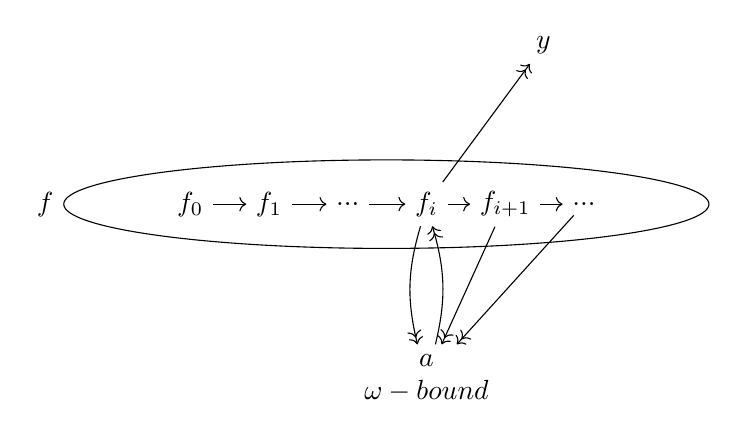
\begin{tikzpicture}
      % Define the nodes inside the region f
      \node (f0) at (0, 0) {$f_0$};
      \node (f1) at (1, 0) {$f_1$};
      \node (fi) at (3, 0) {$f_i$};
      \node (fi+1) at (4, 0) {$f_{i+1}$};
      \node (dots) at (2, 0) {$...$};
      \node (dots2) at (5, 0) {$...$};

      % Draw the arrows between the nodes inside the region f
      \draw[->] (f0) -- (f1);
      \draw[->] (f1) -- (dots);
      \draw[->] (dots) -- (fi);
      \draw[->] (fi) -- (fi+1);
      \draw[->] (fi+1) -- (dots2);

      % Define the region f
      \node[draw, ellipse, fit=(f0) (dots2), label=left:$f$] {};

      % Define the nodes outside the region f
      \node (a) [below=of fi, yshift=-.5cm] {\parbox{2cm}{\centering $a$ \\ $\omega-bound$}};
      \node (y) [above right=of fi, yshift=.5cm] {$y$};

          % Draw the arrows between the nodes inside and outside the region f
          \draw[->>] (fi) to [bend right=15] (a);
          \draw[->>] (a) to [bend right=15] (fi);
          \draw[->>] (fi+1) -- (a);
          \draw[->>] (dots2) -- (a);
          \draw[->>] (fi) -- (y);   
      \end{tikzpicture}
    \end{center}
    Counterexample to:
    \begin{itemize}
      \item ***** DOES NOT WORK ******
      \item RP-$\to$RP 
      \item RP-$\land$WCR$\to$RP \textcolor{red}{NO< NEEDS A NEW CE}
\end{itemize}

\subsection{Other questions}
\begin{enumerate}
  \item If WCR holds, is WN$\downarrow\subseteq$WN ?
  \item Same question for next bullet in 2.2
  \item Same for bullet 3 in 2.2 (but pointwise!)
  \item Do RP- $\land$ WCR imply RP?
\end{enumerate}
\subsection{ARS in Agda}

Important counterexamples:
\begin{enumerate}
  \item $a,b,c,d$ with sinks $a$ and $d$ and a 2-cycle between $b$ and $c$.
  Counterexample to:
  \begin{itemize}
      \item WCR and WN implies CR.
  \end{itemize}
  \item Loop $a \to a$.
  Counterexample to:
  \begin{itemize}
    \item $\omega$-bounded and RP implies SN
    \item $\omega$-bounded and RP implies WN
  \end{itemize}
  \item Infinite sequence $a_0 \to a_1 \to \cdots$. Falsifies:
  \begin{itemize}
    \item $WN$
    \item $\omega$-bounded
    \item RP $\to$ $\omega$-bounded
    \item $WCR \to WN$
    \item $CR \to WN$
    \item $CR, CP \to WN$
    \item $CR, CP \to \omega$-bounded
  \end{itemize}
  \item Infinite sequence $a_0 \to a_1 \to \cdots$ with a colimit $a_\infty$,
  with each $a_n \to a_\infty$ and $a_\infty$ a normal form.

  Counterexample to:
  \begin{itemize}
    \item WN $\to$ SN
    \item WN, CR $\to$ SN
    \item WN, CR, $\omega$-bounded $\to$ SN
  \end{itemize}

  \item Infinite sequence $a_0 \to a_1 \to \cdots$, together with links
  $a_n \to a_0$, for each $n$.
  \item The combination of the last two.
  Counterexample to
  \begin{itemize}
    \item RP
  \end{itemize}
  \item An ``infinite haircomb''. Infinite sequence $a_0 \to a_1 \to \cdots$, together with
  a disjoint, discrete set $b_0, b_1, \dots$, and links $a_n \to b_n$.
  Counterexample to:
  \begin{itemize}
    \item $WN\to WCR$
    \item $WN\to \omega-bounded$
    \item $WN \to SN$
    \item $WN,RP \to SN$
  \end{itemize}
  \item A variation of the above with backlinks $a_n \to a_0$ for all $n$.
\end{enumerate}
\newpage
\newpage
\section{Classical properties}
Principles we are considering
\begin{itemize}
  \item Decidability of equality on $A$
  \item Decidability of the relation $R$
  \item When relevant, decidability of the given precicate $P$
  \item Not-not-closure of being accessible
  \item Not-not-closure of $R$
  \item Not-not-closure of $P$
  \item Decidability of whether a given element is an $R$-normal form
  \item When relevant, local/element-wise versions of the above
  \item Markov's principle:
  \begin{itemize}
    \item In $wfMin_0 \to wfSeq$.

    Given a sequence $s : \nat \to A$, let $E(a) = \exists n \in \nat. s n \equiv a$.

    Need: $\forall a. \lnot\lnot E(a) \to E(a)$, i.e.,
    \[\lnot\lnot \big(\exists n \in \nat. s n \equiv a\big)
          \to \big(\exists n \in \nat. s n \equiv a\big)\]

  \end{itemize}
\end{itemize}
\newpage
\section{Well foundedness }
\begin{enumerate}
    \item For a given element $x$, is the property of
    being accessible $\lnot\lnot$-closed? I.E.,
    Does $x$ being $\lnot\lnot$-accessible imply that $x$ is accessible?
    (Conjecture: No.)
  
    \item As a special case, does being weakly (accessible) well-founded imply being $\lnot\lnot$-wellfounded?
    (Conjecture: No.)
  
    Also: Same question about inductive notion of well-foundedness.
  
    \item ($\star$) Given a well-founded relation, does every non-empty subset
    have a minimal element?
  
    \emph{Problem.} Need to decide whether, for a given $x \in U$,
     the set $\{y | Ryx\}$ is empty.
  
     \item IF every non-empty subset has a minimal element, does this imply
     either of the weak forms of well-foundedness: $\mathtt{isWFacc-}$ or
     $\mathtt{isWFind-}$ ?
  
     \item Does $\mathtt{isWFmin-}$ imply $\mathtt{isWFacc-}$ or $\mathtt{isWFind-}$?
  
     \emph{Problem.} Need to go from $\lnot (\forall y. R y d \to \phi y)$
     and $\forall y. R y d \to \lnot \lnot \phi y$ to $\bot$.
  
     In terms of accessibility, it should suffices to assume accessibility is
     $\lnot\lnot$-closed, since being related to y is not relevant for that. (?)
  
     \item Does sequential well-foundedness (no decreasing sequence) imply
     any of the other notions, e.g., \texttt{WFmin-} ?
  
     \emph{Note.}  This seems to require the most classical assumptions:
     $\lnot\lnot$-closure of $\phi$, relativized De Morgan law,
     Markov's principle, etc.
  
     
  
  \end{enumerate}
  
  \textsc{Remark.}
  $\lnot\lnot$-closure of accessibility should solve problems 1 and 4.
  
\newpage
\section{Guide to the code}
\section{Open problems}
\begin{itemize}
    \item Look at restricting WFmin to $\lnot\lnot$-closed predicates
    \item Status of important hypotheses:
      \begin{itemize}
        \item Deciding whether a given element $x$ reduces to a given element $y$
        (Is $R$ itself decidable?)
        \item Deciding whether a given element $x$ reduces to some element $y$
        (Is being an $R$-normal form decidable?)
  
        {\textcolor{red}{This is needed to show that SN $\Rightarrow$ WN.}}
  
        \item If a given element $x$ is \emph{not} a normal form,
        exhibiting some element $y$ that it reduces to.
        (This is related to DeMorgan/Markov/etc. properties that came up in WF file.)
  
        \item Does UN-lemma \emph{require} the decidability assumption?
      \end{itemize}
    \item META questions: Which of the ARS theorems can be made ``local/pointwise'',
    for example,
    \begin{itemize}
      \item NL+: $WCR(R) \land SN(x) \to CR(x)$?  (Yes?)
      \item NL++: $WCR(x) \land SN(x) \to CR(x)$? (No.)
    \end{itemize}
    \item When time permits, uniformize the notation (variable names, etc.) to the extent possible.
    \item Can "sequential" properties like RP, RP-, isWFseq, isWFseq-, $\omega$-bounded, etc.,
    be related to the cofinality property.
    \item What happens if properties involving sequences are reformulated for
  $R^r$? (Cannot decide whether the given sequence is finite or infinite.)
  \item Knaster-Tarski Lemma: Most general form? Alternative formulations?
  \item Syntax for closure operators allowing to prove the needed properties
  uniformly/generically
  \item More laws about closure operations: Monotonicity, idempotency
  \item \item Knaster--Tarski in a well-founded setting: what additional
  hypotheses are necessary?
  \item (2024.10.10) Is being $R$-WN inductive?
    \item (2024.10.10) Does $R$ being finitely branching imply
     that, for an inductive $\phi$, if $\lnot \phi(x)$ then
     $\exists y. Rxy \land \lnot \phi(y)$?

     \item The infinite haircomb refutes $WN \land RP \to \omega$-bounded.  But it is not WCR.

     So, does $WN, RP, WCR$ imply $\omega$-bounded?
     Answer: yes, that is what we have proved classically.
   
     \item Wait, does RP- actually imply RP????
   
     \item RP- and $\omega$-bounded implies RP?
     \item RP- and WCR imply RP?
     \item
     \[ WNg \land UN \to CRelem :
     \forall (R : \mathscr{R} A) \to WN R \to \forall x \to is R -UN x \to is R -CR x \]
     \item $WN R \to UN R \to \omega-bdd R \to SN R$ (1.2.3.ii-)
      \item Finish formulating the ``compactness property".  Two candidates:
       \item ``Every cocone for a given infinite sequence loops back to some point in the sequence"
       \item ``If an $R^*$-sequence has a cocone then it's constant after some point on.''
       \item is $\omega$-bounded implied by WN and the following confluence property:
       $a \to^* n \in NF$, and $a \to b$ then $b \to^* n $.
    \item  Make the first argument to "being a normal form" implicit?
    \item Write up the classical proof to theorem 1-2-3 iii
     

\end{itemize}
\section{Conclusions}






\end{document}